\newpage

\section{Reproducing stylized facts with HMMs}
\label{Section: Stylized facts}
As highlighted throughout section \ref{section: Data} the normal distribution provides a poor fit for financial returns. Furthermore, financial returns are characterised by a set of stylized facts. Researchers including Granger \& Ding (1995b), Cont (2001) and Malmsten \& Teräsvirta (2010) have found a variety of different stylized facts that are persistent across asset returns. In addition, Rýden et al. (1998) showed the how HMMs can reproduce most of the stylized facts, in which the analysis was rooted on daily returns of the S\&P 500. Rýden et al. (1998) found that most of the stylized facts could in fact be reproduced by a HMM, however, the slow decay characterising the  squared autocorrelation function of daily returns, which is of great importance in financial risk management, could not be reproduced satisfactorily. More recently, Nystrup (2017) showed promising results in terms of HMMs reproducing the the squared autocorrelation function, albeit not achieving a perfect fit. 

The data analyzed in this thesis encompass daily returns of the S\&P 500 stock index from 1960 to 2021. As such, the predominant amount of the time series data used by the above-mentioned authors, is represented in the data underlying this thesis. Despite the unanimity in the overall methodology of the studies conducted by the aforementioned authors there are differences in their respective objectives. For instance, Granger \& Ding (1995b) divided the time series data into ten subsamples of 1,700 observations, which corresponds to a little less than seven years. Granger \& Ding (1995b) worked under the assumption that it was likely that with such a long time span there could have been structural shifts in the datagenerating process. Using a similar approach, Rydén (1998) found that the estimated HMMs, including the number of states and the type of conditional distributions, changed considerably between the subsamples.

As such, this section will be reserved for training HMMs through the aforementioned MLE and JUMP methodology, after-which the corresponding models serve as subject for analysis of how well they reproduce the stylized facts. The methdology outlined in this section will take a great amount of inspiration from Granger \& Ding (1995), Rýden et al. (1998) as well as Nystrup (2017).

\subsection{Rolling estimation}
Rýden et al. (1998) relied on a methodology in which a Gaussian HMM is estimated for ten subseries of a log return series generated from 17,000 daily observations from the S\&P 500 index. This methodology also closely follows the methodology originally put forward by Grangner \& Ding (1995b). In recent publications Bulla (2011) and Nystrup (2014) rely on estimating univariate HMMs through a rolling window of (1000 or 2000) trading days. This will result in ($\text{Number of observations} - 2000$) models being estimated, which thereby allows for capturing the time-varying nature of the HMMs' parameters. The advantage of Nystrup's methodology is the fact that the rolling window allows for gradually forgetting previous observations when estimation the models, whereas the subset methodology presented by Granger \& Ding estimates 10 unique HMMs from non-overlapping observations from the return series. 

As highlighted in section \ref{section: Data} this thesis relies on daily observations due to the favorable properties associated with early detection. The explanatory variable will be the daily returns of the S\&P 500 index, thereby making the results somewhat comparable to the aforementioned authors. It should be noted that it is not important whether the explanatory variable tradeable as it will purely be used for signalling regime changes. Stock indices and yield spreads both serve as popular explanatory variables as they tend to lead the economy (Dungey et al, 2000). Essentially this means that stock indices and yield spreads will exhibit local maxima/minima approximately around the time of an economic regimes change. As such, both are suitable indicators, however, to increase comparability to the aforementioned literature, stock indices, and more precisely, the S\&P 500 index is preferred. 

As emphasized in section \ref{section: estimation}, this thesis aims at comparing the properties of the MLE and JUMP estimation procedure, in which a vital part of comparing and determining the most viable estimation methodology revolves around the methodology's capability of reproducing the stylized facts associated with asset returns. For this section the thesis will estimate 2-state univariate Gaussian HMMs through the MLE and JUMP methodology using a rolling window of XXXX trading days. That is, for each time step $t$ a HMM is estimated by the MLE and JUMP approach using the previous XXXX log returns, as the model parameters are stable at this length. Furthermore, the chosen window length makes it appropriate to compare results against those of Bulla (2011) and Nystrup (2014), albeit these authors neglect estimation the HMMs through the JUMP framework. After origination the rolling window moves one time period forward to $t+1$ iteratively. The choice of the number of trading days for regarding window length is based on the aforementioned authors which all select a rolling window length between 1000 and 2000 days. Essentially, the window length is a hyperparameter that can be tuned and the exact choice boils down to a trade-off relationship between bias and variance. A shorter rolling window will, all else equal, result in a faster adaption to changes in the underlying economic regimes but the estimate will be more noisy as fewer observations are used when deriving the parameters. This might result in the model adapting to "wrong" signal, which might affect the underlying trading strategy by decreasing risk-adjusted returns. A range of rolling window days have been tested and can be found in appendix XXX.

The results of the rolling parameter for the MLE and JUMP estimation of the 2-state Gaussian HMMs are shown in figure XXX and YYY repsectively. The dashed lines are the maximum likelihood estimate when the model is shown the entire batch of observations i.e. if one were to assume that the parameters underlying the HMM were static. 

\begin{figure}[H] 
    \centering
    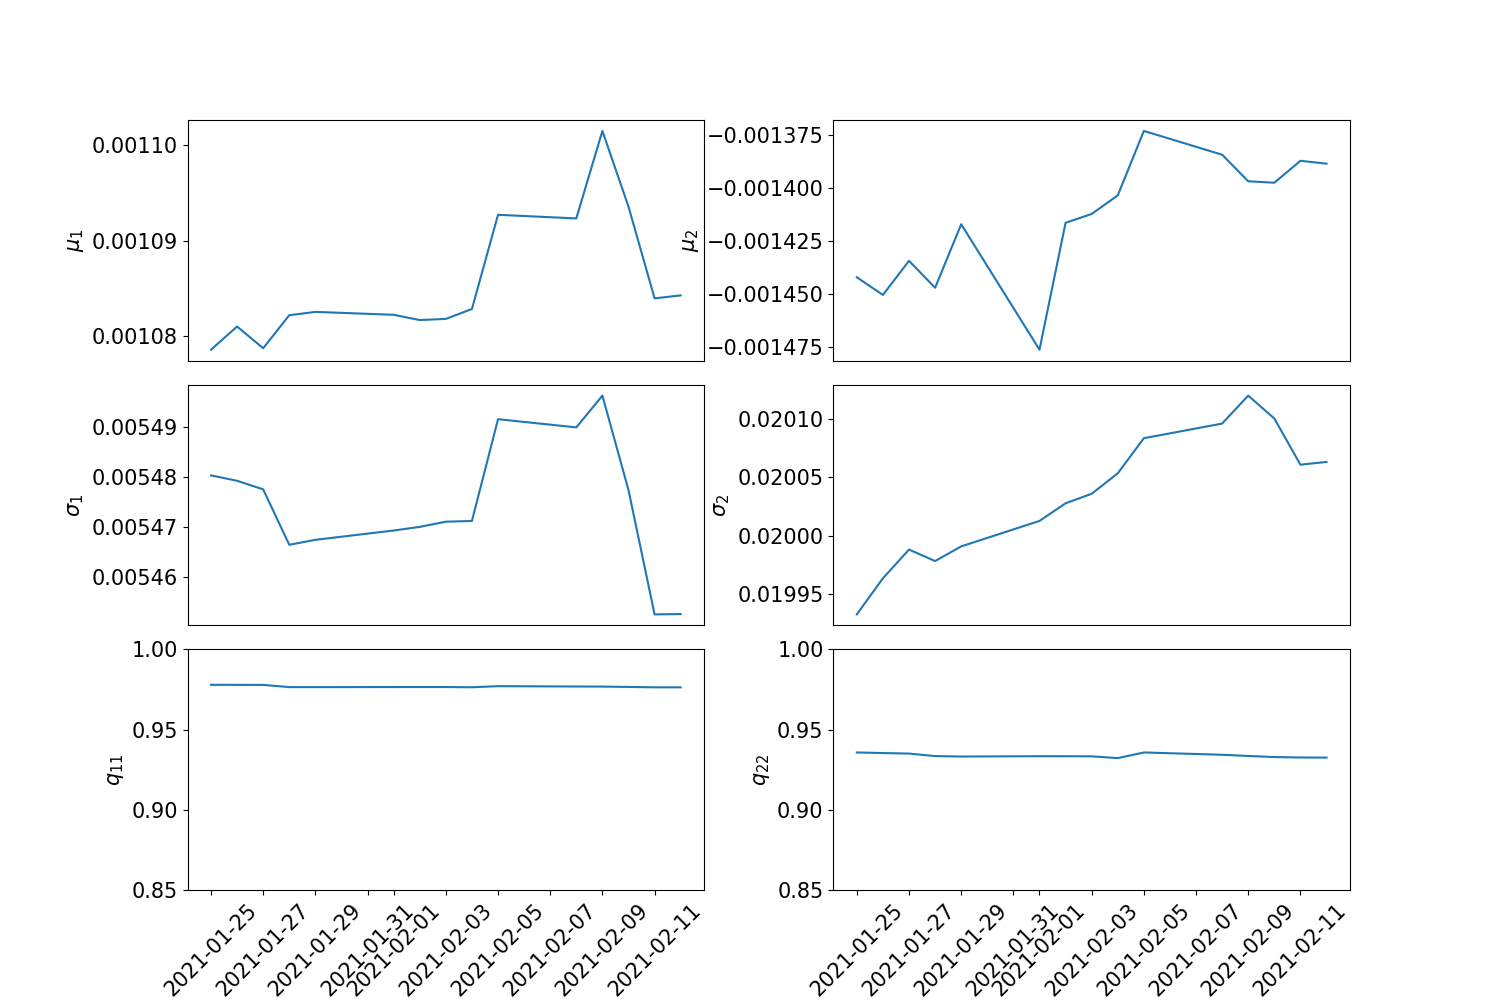
\includegraphics[width=1.0\textwidth]{analysis/stylized_facts/2-state MLE HMM rolling params.png}
    \caption{Rolling estimation based on the MLE approach. Parameters from a 2-state Gaussian HMM using a rolling window of XXX days. The size of the estimation window is particularly visible in the bear state where $\sigma_2^2$ significantly increase after the financial crisis, and only drops back down to pre-crisis levels after approximately XXX days. Dashed lines are parameters from an HMM estimated on the full sample.}
    \label{fig: MLE estimation rolling parameters} 
\end{figure}

\begin{figure}[H] 
    \centering
    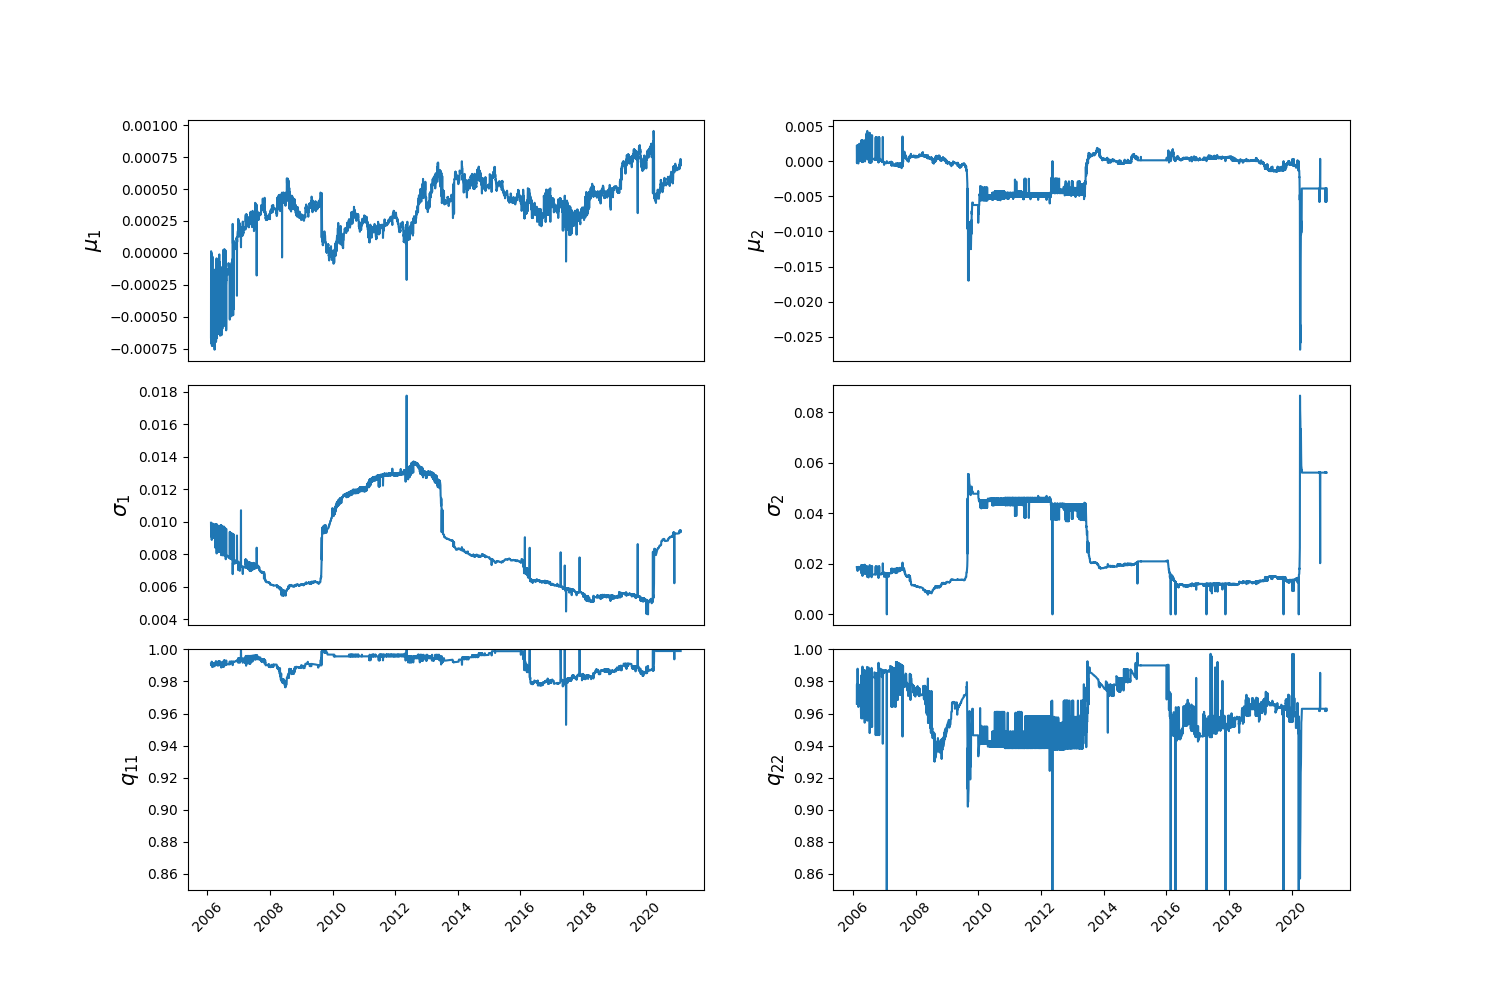
\includegraphics[width=1.0\textwidth]{analysis/stylized_facts/2-state JUMP HMM rolling params.png}
    \caption{Rolling estimation based on the JUMP approach. Parameters from a 2-state Gaussian HMM using a rolling window of XXX days.}
    \label{fig: Jump estimation rolling parameters} 
\end{figure}

From figure \ref{fig: MLE estimation rolling parameters} and \ref{fig: Jump estimation rolling parameters} it is evident that neither the mean nor variance parameters exhibit stationarity across time
for the 2-state Gaussian HMM regardless of whether the estimation procedure relies on MLE or JUMP. Starting with the MLE approach showcased in figure \ref{fig: MLE estimation rolling parameters} it becomes eveident that around the global financial crisis an interesting pattern emerges since $\sigma_2^2$ drastically increased after-which it appears that the parameter falls back to its original pre-crisis level after XXX days. As such, it is peculiar that $\sigma_2^2$ should decreases almost XX years later, where the observations witnessed during the GFC gets dropped due to the length of the chosen rolling window. This could imply that the bear state fluctuates around some long-run level, in which large deviations only occur for extreme events such as the financial crisis and the COVID-19 recession. 

When analysing the non-constant transition probabilities resulting from the MLE approach in figure \ref{fig: MLE estimation rolling parameters} it can easily be inferred that the sojourn times are not memoryless. Throughout the plot, the bull market has a high persistence, meaning that there is a high probability of a bull market being followed by an additional bull market. Keep in mind that the model is still operating on a daily timescale, thus the finding is expected. Contrary, the transition probabilities of the bear market, i.e. $\sigma_2^2$ and its inverse, are characterised by a higher degree of fluctuations across time. The fluctuations become evident during the GFC, the big market correction of 2016 as well the recent COVID-19 bounce since the probability of staying in the bear market decreases, whilst the probability of remaining in the bull state is more or less unaffected, with the exception of the correction in 2016. This means that the HMM will predict much shorter sojourn times in the bear state, thereby implying that the predictions will be characterised as much more volatile than for instance the bull state predictions. This is a natural consequence of the properties of the transition probabilities because when $q_{22}$ decreases $q_{21}$ increases as $q_{22} + q_{21} = 1$, hence a low value of $q_{22}$ will result in more frequent transitions between states. As such, the persistence of the model will be worse in these periods and it is a clear sign of model weakness, as it will impact the temporal properties by reducing the fit to the empirical squared autocorrelation functions of returns and thus negatively impact the reproduction of the long memory of financial markets. 

In addition, it is evident from the JUMP estimation showcased in figure \ref{fig: Jump estimation rolling parameters} that this methodology also captures the time-varying nature of the underlying HMM parameters. 

Furhtermore, it is evident that there exists some differences between the MLE and JUMP approach.....


. 




\subsection{Distributional properties}

\textbf{Train a number of models and compare their first 4 moments to those of S\&P500. Also show distributional properties as a function of time i.e. the 4 moments across time (see BP)}

\textbf{Add outlier corrected graphs. Consider if outlier corrections should be done on a rolling basis or a one-off procedure on full dataset}

\begin{figure}[H] 
    \centering
    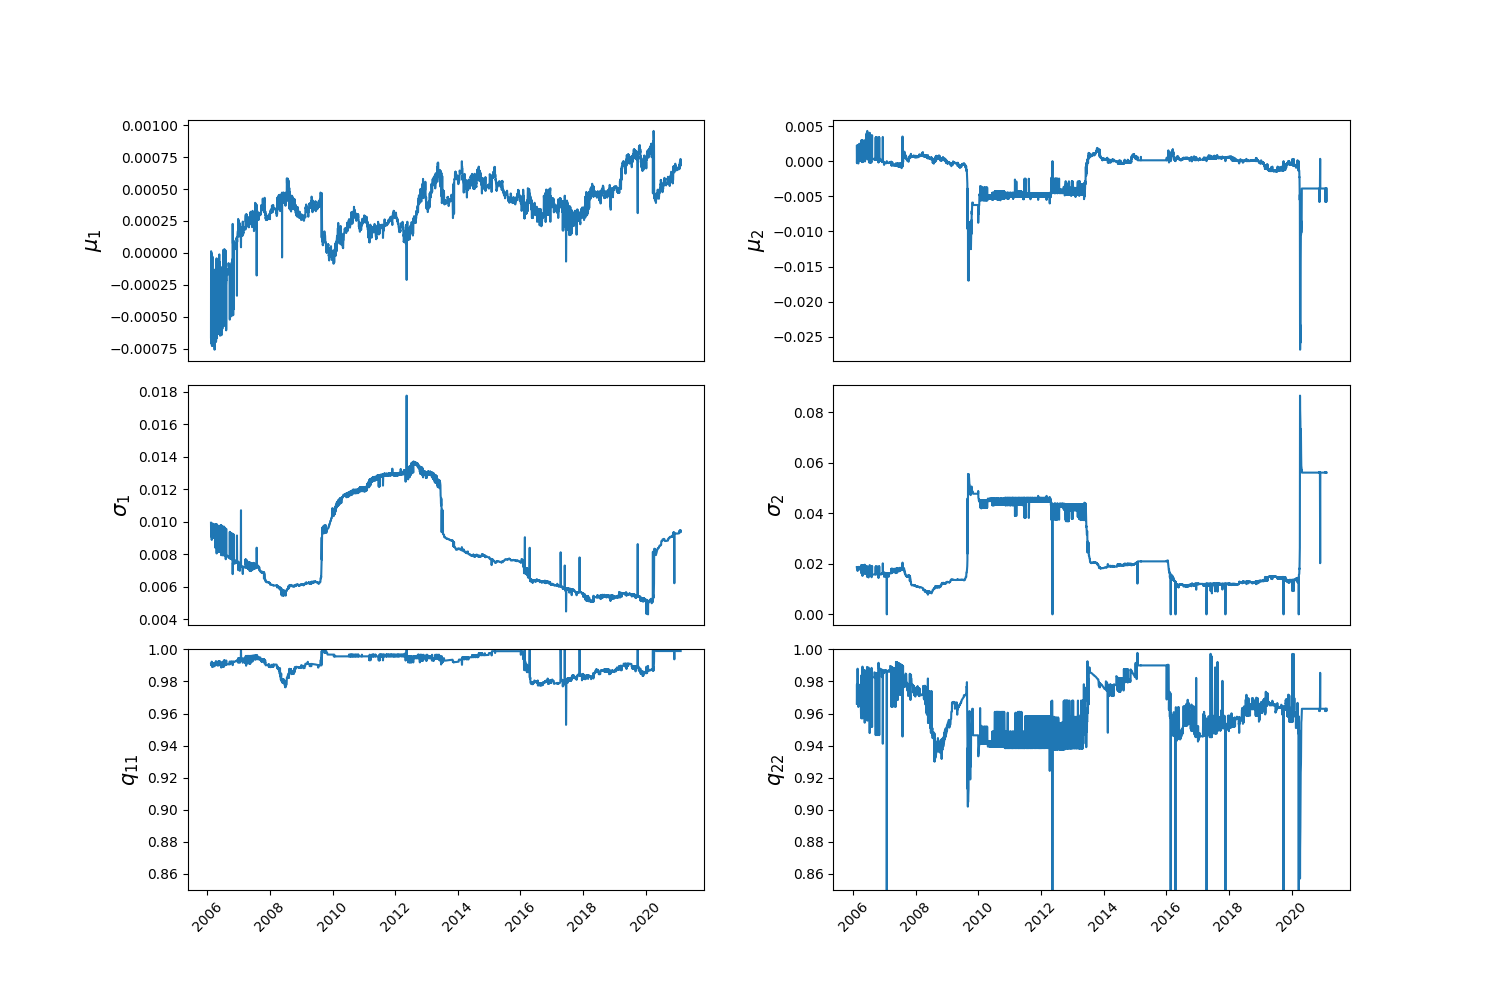
\includegraphics[width=1.0\textwidth]{analysis/stylized_facts/2-state JUMP HMM rolling params.png}
    \caption{Development of first four moments of estimated models compared to $\log(r_t)$ using a rolling window of 1700 days. Model estimates are calculated using Monte-Carlo simulations.}
    \label{fig:stylized_facts_rolling_moments} 
\end{figure}


\subsection{Temporal properties}

\textbf{Show ACF plots of same figures as in previous section}

\begin{figure}[H] 
    \centering
    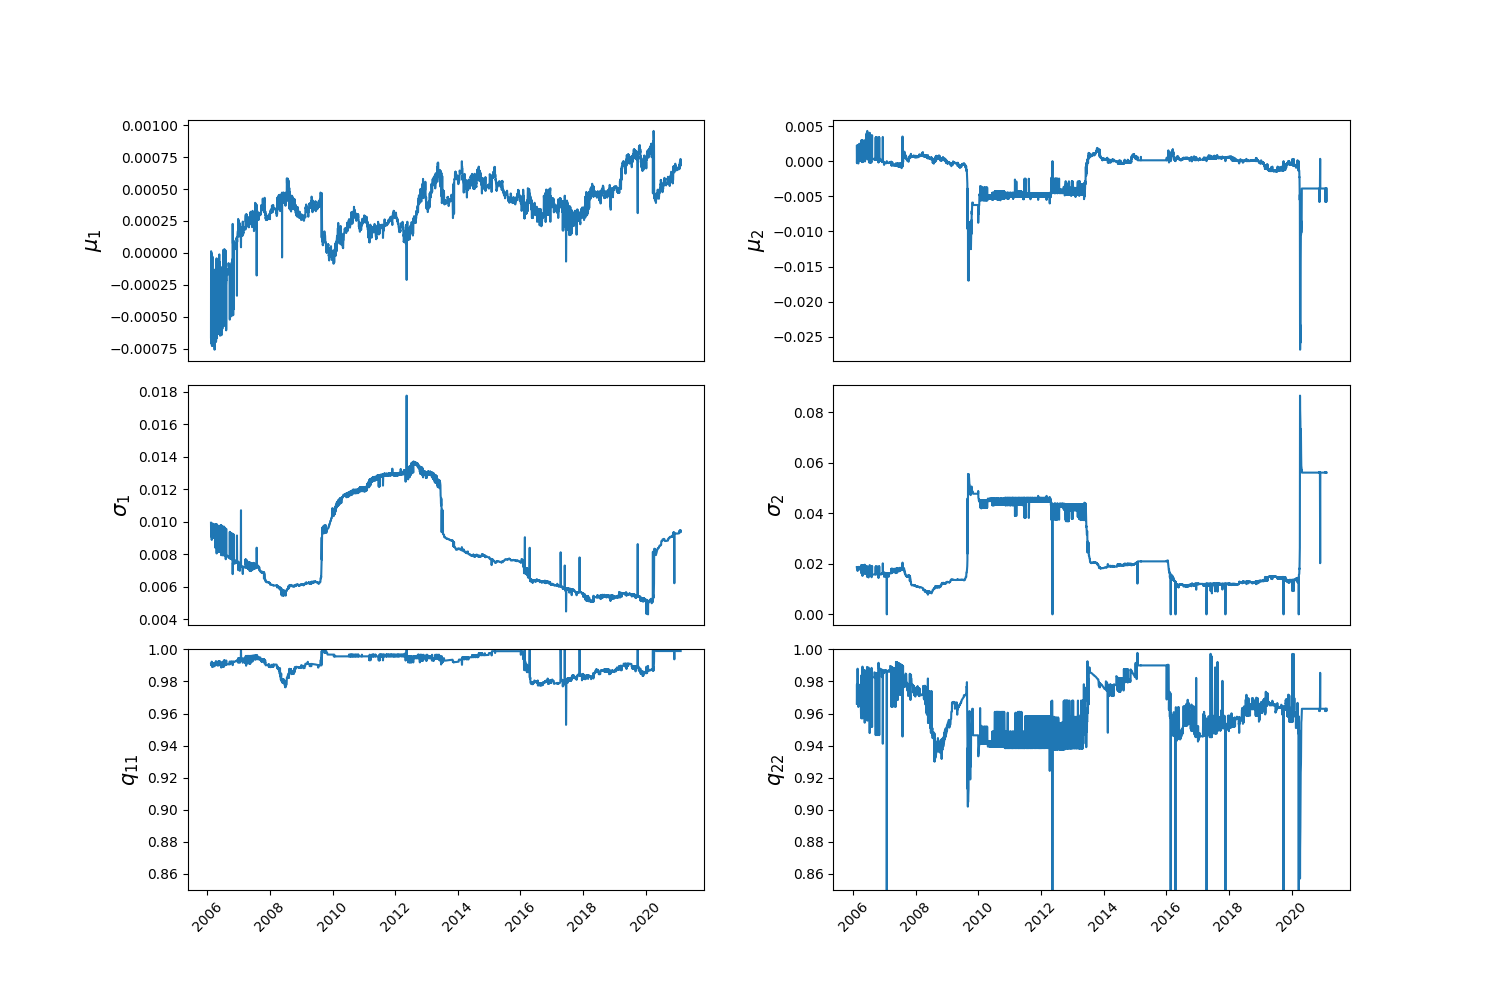
\includegraphics[width=1.0\textwidth]{analysis/stylized_facts/2-state JUMP HMM rolling params.png}
    \caption{Development of first four moments of estimated models compared to $\log(r_t)$ using a rolling window of 1700 days. Model estimates are calculated using Monte-Carlo simulations.}
    \label{fig:stylized_facts_acf_plots} 
\end{figure}

\subsection{Smoothing}

\textbf{If smoothing works, then show distributional properties and temporal proerties again.}

\textbf{Show decoded states on times series}

\subsection{Model estimation and selection}
\label{Subsection: Model estimation and selection}
